% L9c convexity figure, two panels. Left: a convex loss, a tilted parabola, where
% the chord between f(a) and f(b) lies above the graph. Right: the gradient
% descent schematic's loss, where the graph rises above the chord between the
% local minimum theta_2 and the lower minimum theta_1.
%
% Drawn on October 22, 2026 with the gradient descent schematic's palette.
%
% Left curve: y = 0.35 s^2 rotated by 20 degrees about its vertex V, so the bowl
% rises gently on the left and steeply on the right. The rotated curve stays a
% graph for s < cos(20)/(2*0.35*sin(20)) = 3.92. V was placed so the lowest
% point (s = -tan(20)/0.70 = -0.520) sits at (6.40, 0.80); the domain ends where
% the curve reaches y = 5.60. Points computed from the same parametrization:
%   a: s = -3.782 -> (1.655, 4.300)
%   b: s =  2.125 -> (8.377, 3.100)
%   t = 1/2: x = 5.016, chord 3.700, curve 1.236
%
% Right curve: the four cubic Bezier segments of Fig-GD-Schematic, so theta_2
% (1.40, 2.30), the hump (2.80, 2.95), and theta_1 (5.60, 0.65) are the same
% points. The chord at the hump is 2.30 - (1.40/4.20)(1.65) = 1.75.
%
% Math uses the standard TeX fonts (no unicode-math), so \theta renders as the
% same plain theta the notebook's math shows.
%
% The notebook SVG carries a dark palette added by theme_svg.py; keep new
% colors in that script's mapping when changing the palette here.
\documentclass[tikz,border=4pt]{standalone}
\usepackage[no-math]{fontspec}
\IfFontExistsTF{Arial}{\setsansfont{Arial}}{\setsansfont{TeX Gyre Heros}}
\renewcommand{\familydefault}{\sfdefault}
\usepackage{amsmath,amssymb}
\usetikzlibrary{arrows.meta,calc}

% Same colors as Fig-GD-Schematic.
\definecolor{vnink}{HTML}{202124}
\definecolor{gdblue}{HTML}{0091FF}
\definecolor{gdred}{HTML}{E02020}
\definecolor{gdgray}{HTML}{6D7278}

\begin{document}
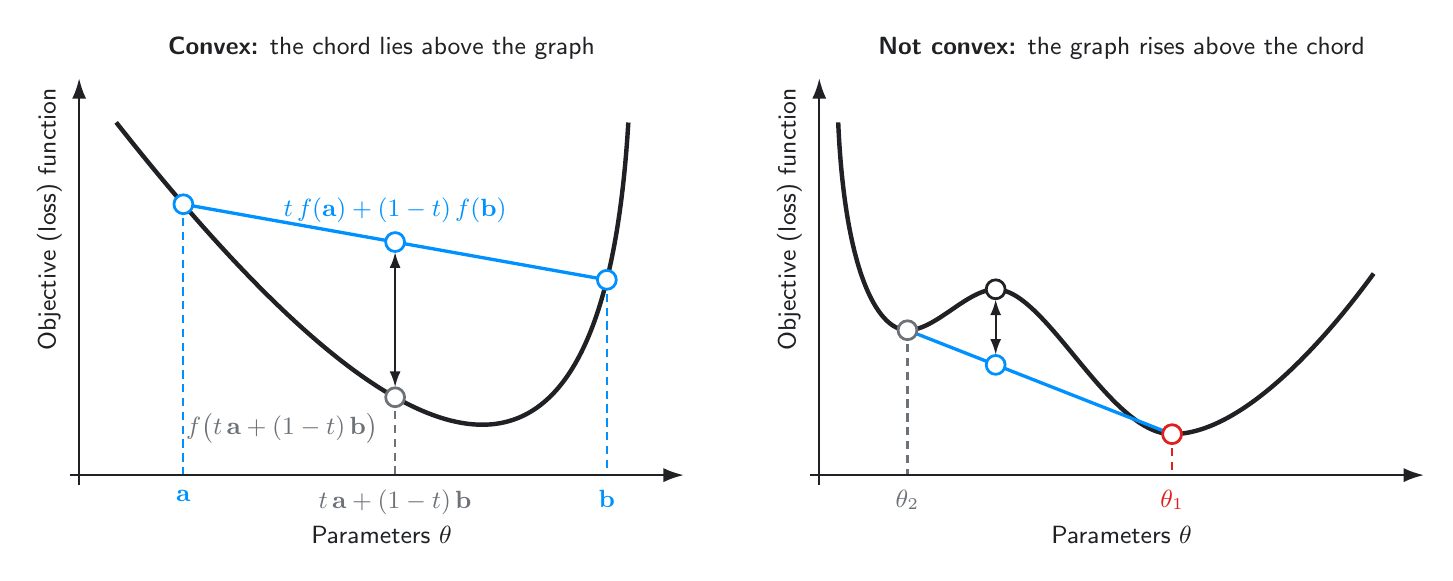
\begin{tikzpicture}[x=0.8cm, y=0.8cm, font=\sffamily\small, text=vnink,
    axis/.style={draw=vnink, line width=0.8pt, -{Latex[length=2.6mm, width=1.8mm]}},
    loss/.style={draw=vnink, line width=1.6pt},
    chord/.style={draw=gdblue, line width=1.2pt},
    drop/.style={line width=0.8pt, dash pattern=on 3pt off 2pt},
    gap/.style={draw=vnink, line width=0.8pt, {Latex[length=2.0mm, width=1.4mm]}-{Latex[length=2.0mm, width=1.4mm]}},
    pt/.style={circle, fill=white, line width=1.0pt, inner sep=0pt, minimum size=2.4mm},
  ]

  % ---------------- left panel: convex ----------------
  \begin{scope}
    \coordinate (a) at (1.655, 4.300);
    \coordinate (b) at (8.377, 3.100);
    \coordinate (mc) at (5.016, 3.700);  % chord at t = 1/2
    \coordinate (mf) at (5.016, 1.236);  % curve at t = 1/2

    \draw[drop, gdblue] (a) -- (a |- 0,0);
    \draw[drop, gdblue] (b) -- (b |- 0,0);
    \draw[drop, gdgray] (mf) -- (mf |- 0,0);

    \draw[axis] (-0.15, 0) -- (9.6, 0);
    \draw[axis] (0, -0.15) -- (0, 6.3);
    \node[anchor=north] at (4.8, -0.65) {Parameters $\theta$};
    \node[rotate=90, anchor=south east] at (-0.12, 6.3) {Objective (loss) function};
    \node[anchor=south] at (4.8, 6.45) {\textbf{Convex:} the chord lies above the graph};

    \draw[loss] plot[domain=-4.340:3.300, samples=150, variable=\s]
      ({6.921 + \s*cos(20) - 0.35*\s*\s*sin(20)}, {0.889 + \s*sin(20) + 0.35*\s*\s*cos(20)});
    \draw[chord] (a) -- (b);
    \draw[gap] ($(mc) + (0, -0.16)$) -- ($(mf) + (0, 0.16)$);

    \node[anchor=north, text=gdblue] at (a |- 0,-0.08) {$\mathbf{a}$};
    \node[anchor=north, text=gdblue] at (b |- 0,-0.08) {$\mathbf{b}$};
    \node[anchor=north, text=gdgray] at (mf |- 0,-0.08) {$t\,\mathbf{a}+(1-t)\,\mathbf{b}$};
    \node[anchor=south, text=gdblue] at ($(mc) + (0, 0.15)$) {$t\,f(\mathbf{a})+(1-t)\,f(\mathbf{b})$};
    \node[anchor=north east, text=gdgray] at ($(mf) + (-0.12, -0.10)$) {$f\bigl(t\,\mathbf{a}+(1-t)\,\mathbf{b}\bigr)$};

    \node[pt, draw=gdblue] at (a) {};
    \node[pt, draw=gdblue] at (b) {};
    \node[pt, draw=gdblue] at (mc) {};
    \node[pt, draw=gdgray] at (mf) {};
  \end{scope}

  % ---------------- right panel: not convex ----------------
  \begin{scope}[xshift=9.4cm]
    \coordinate (t2) at (1.40, 2.30);
    \coordinate (t1) at (5.60, 0.65);
    \coordinate (hc) at (2.80, 1.75);  % chord below the hump
    \coordinate (hf) at (2.80, 2.95);  % top of the hump

    \draw[drop, gdgray] (t2) -- (t2 |- 0,0);
    \draw[drop, gdred] (t1) -- (t1 |- 0,0);

    \draw[axis] (-0.15, 0) -- (9.6, 0);
    \draw[axis] (0, -0.15) -- (0, 6.3);
    \node[anchor=north] at (4.8, -0.65) {Parameters $\theta$};
    \node[rotate=90, anchor=south east] at (-0.12, 6.3) {Objective (loss) function};
    \node[anchor=south] at (4.8, 6.45) {\textbf{Not convex:} the graph rises above the chord};

    \draw[loss] (0.30, 5.60) .. controls (0.40, 3.30) and (0.90, 2.30) .. (1.40, 2.30)
      .. controls (1.85, 2.30) and (2.35, 2.95) .. (2.80, 2.95)
      .. controls (3.60, 2.95) and (4.60, 0.65) .. (5.60, 0.65)
      .. controls (6.70, 0.65) and (8.00, 2.10) .. (8.80, 3.20);
    \draw[chord] (t2) -- (t1);
    \draw[gap] ($(hf) + (0, -0.16)$) -- ($(hc) + (0, 0.16)$);

    \node[anchor=north, text=gdgray] at (t2 |- 0,-0.08) {$\theta_{2}$};
    \node[anchor=north, text=gdred] at (t1 |- 0,-0.08) {$\theta_{1}$};

    \node[pt, draw=gdgray] at (t2) {};
    \node[pt, draw=gdred] at (t1) {};
    \node[pt, draw=gdblue] at (hc) {};
    \node[pt, draw=vnink] at (hf) {};
  \end{scope}
\end{tikzpicture}
\end{document}
